Using the likelihood from the previous section, we perform a maximum likelihood fit to the observed \ETg\ distributions in all the control samples and signal region simultaneously.
The minimization of the negative log likelihood is performed using the Minuit2 algorithm through an interface provided in the RooStats package ~\cite{RooStats2010}.

\begin{figure}[htbp]
  \centering
  \resizebox{\textwidth}{!}{
    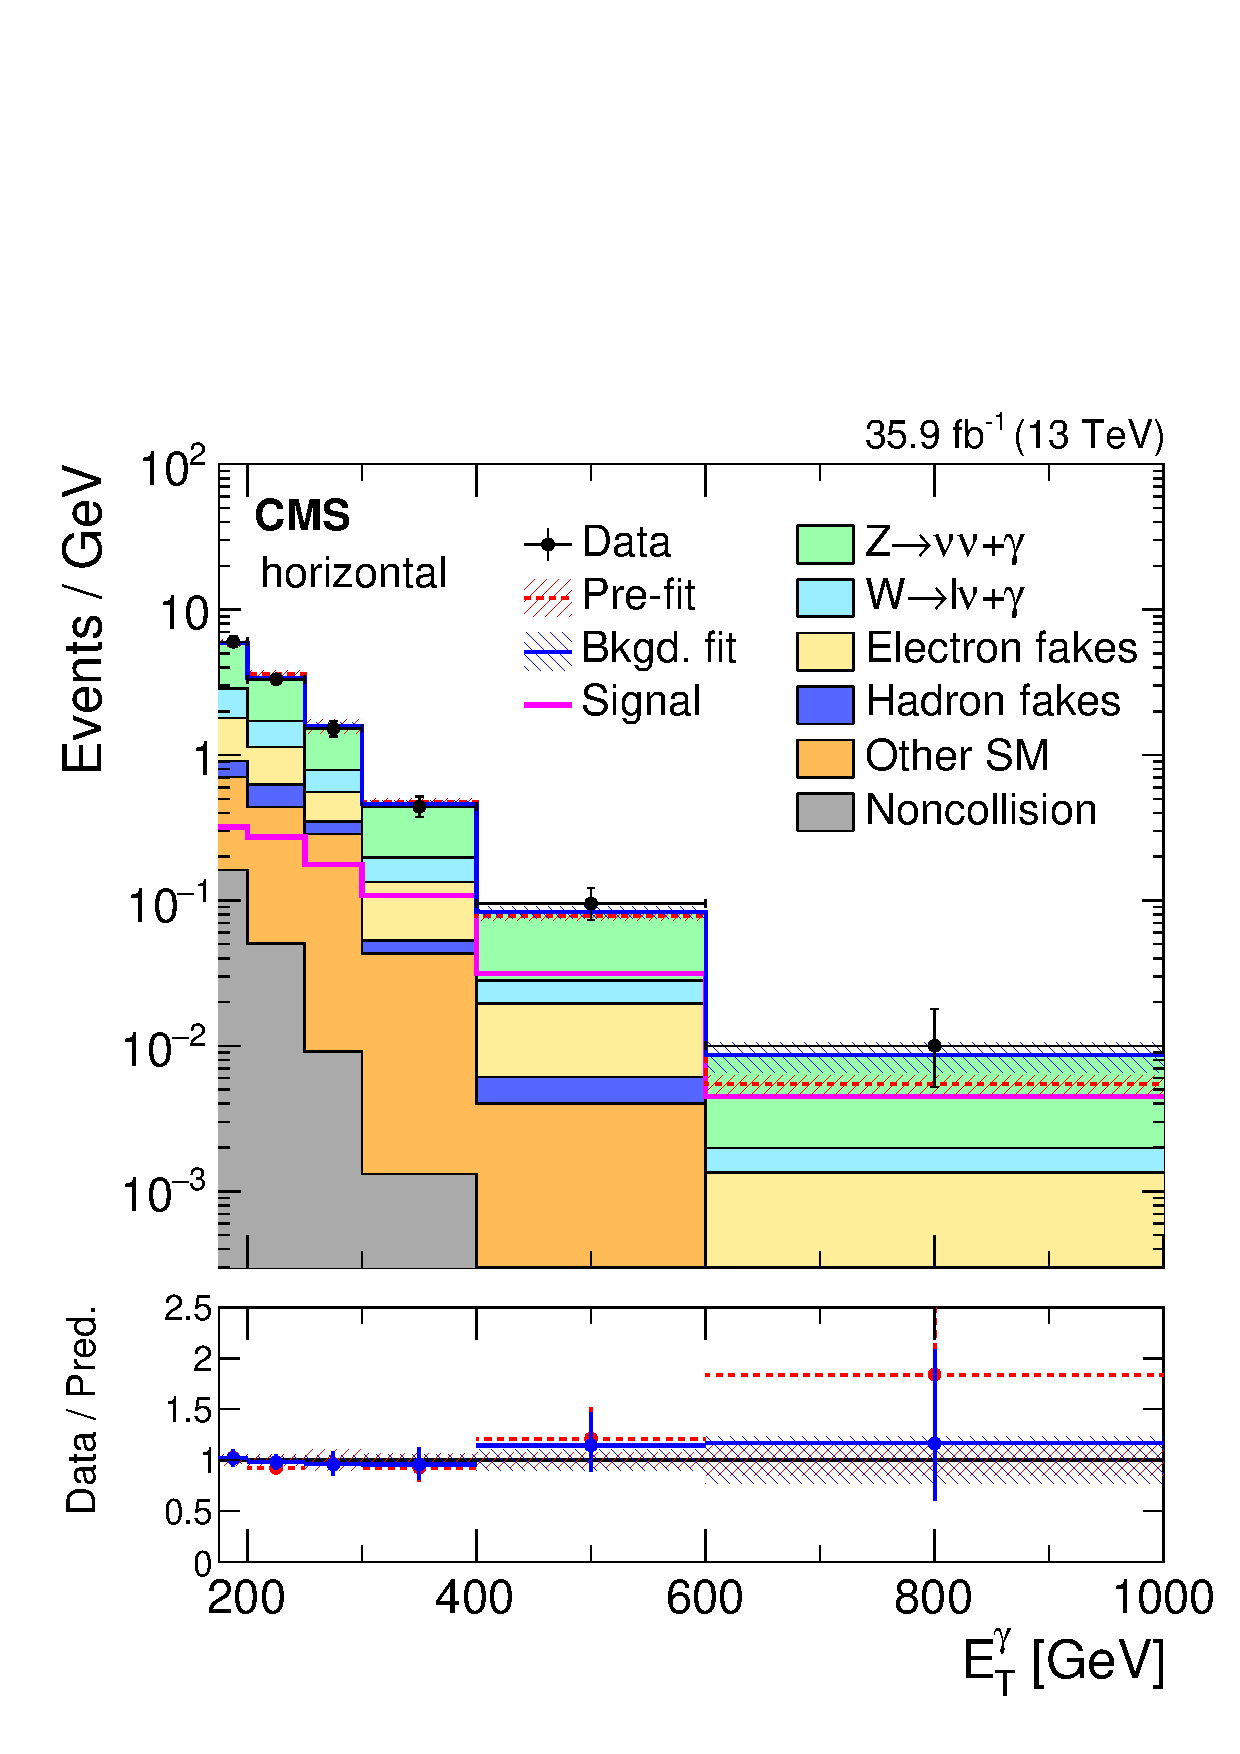
\includegraphics[]{Analysis/Figures/bonly_horizontal.pdf}
    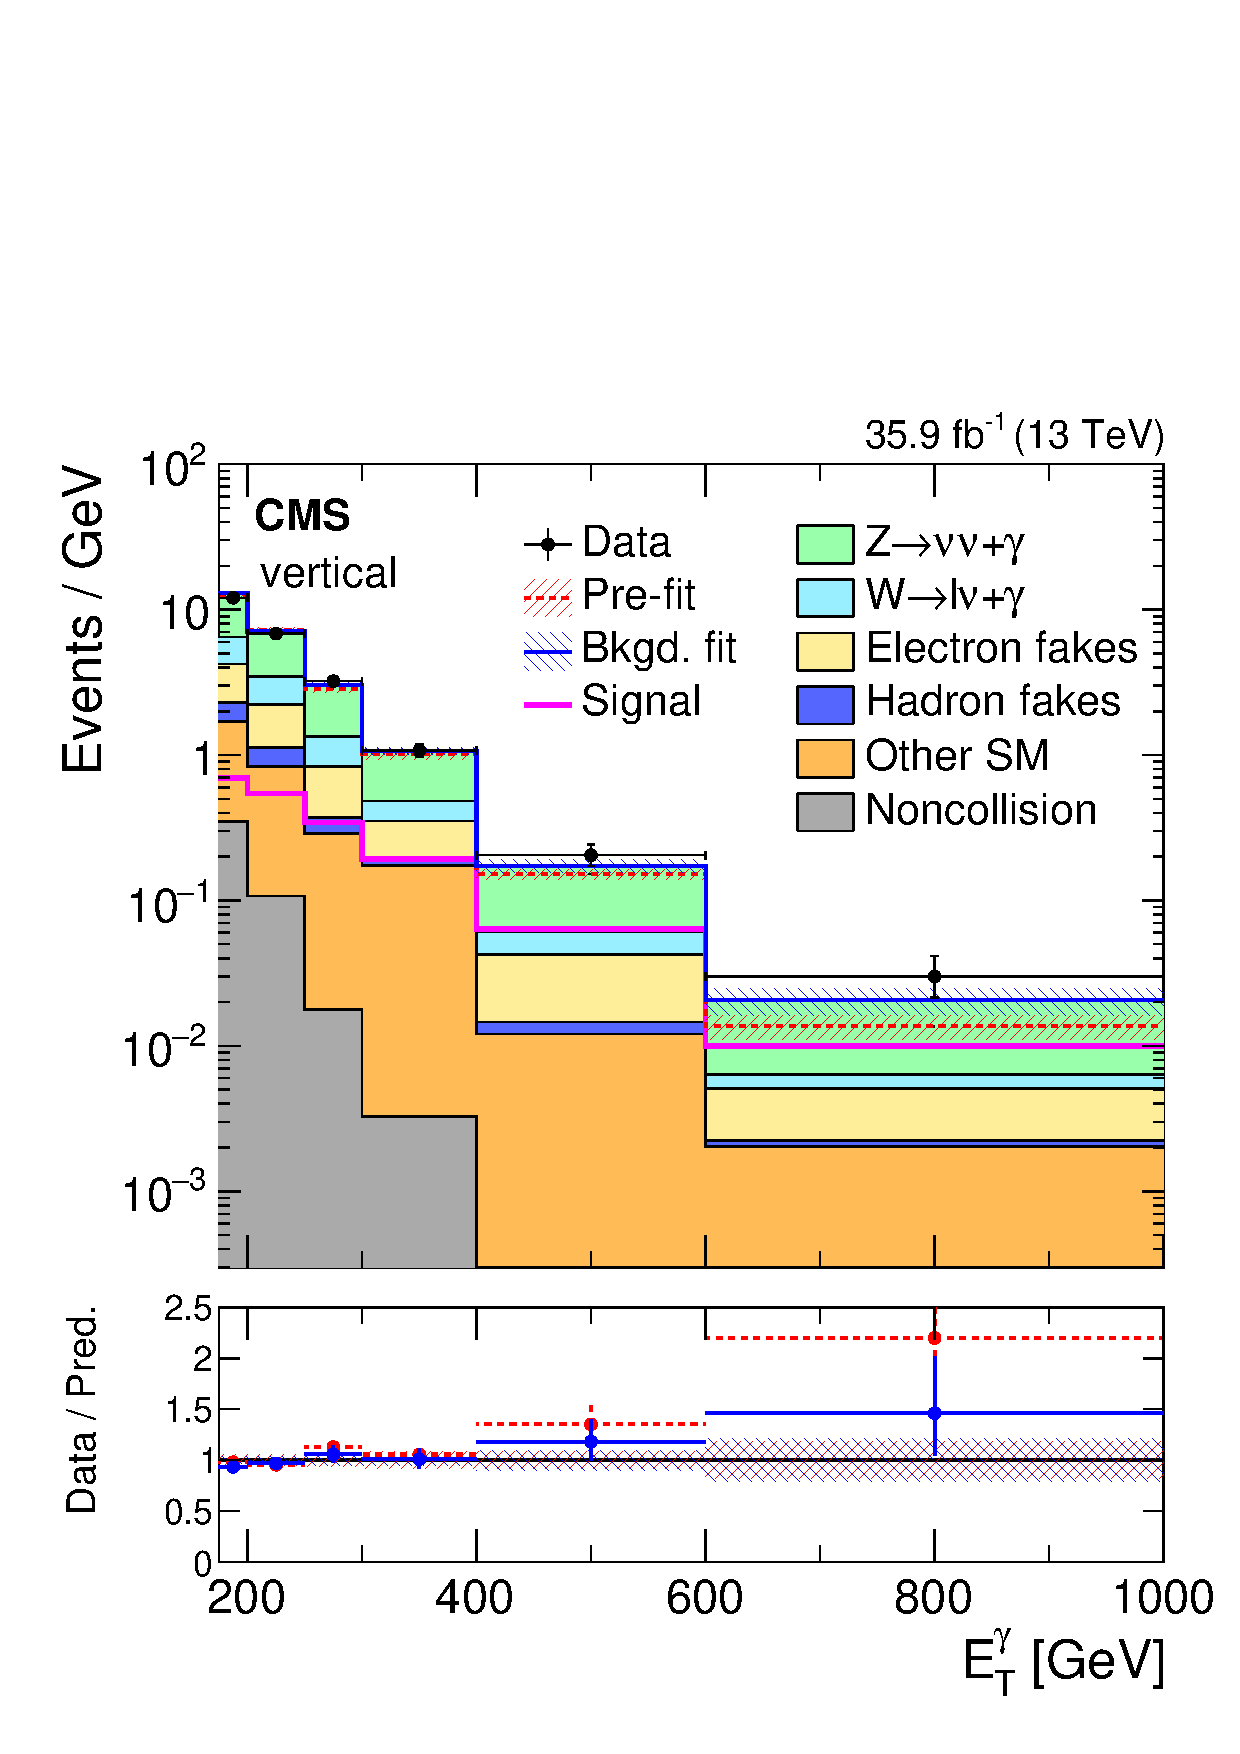
\includegraphics[]{Analysis/Figures/bonly_vertical.pdf}
  }
    \caption{
      Observed \ETg\ distributions in the horizontal (left) and vertical (right) signal regions compared with the post-fit background expectations for various SM processes.
      The last bin of the distribution includes all events with $\ETg > 1000\GeV$. 
      The expected background distributions are evaluated after performing a combined fit to the data in all the control samples and the signal region. 
      The ratios of data with the pre-fit background prediction (red dashed) and post-fit background prediction (blue solid) are shown in the lower panels. 
      The bands in the lower panels show the post-fit uncertainty after combining all the systematic uncertainties. 
      The expected signal distribution from a 1\TeV vector mediator decaying to 1\GeV DM particles is overlaid.
    }
    \label{fig:postfitSR}
\end{figure}

The comparison between the observed distributions and the results from simulations before and after performing the simultaneous fit are shown in Figures~\ref{fig:postfitSR} and~\ref{fig:postfitCR} for the signal and control regions, respectively.
The observed distributions are in agreement with the prediction from SM and non-collision backgrounds and no significant excess of events beyond the SM expectation is observed.

\begin{figure}[htbp]
  \centering
  \resizebox{\textwidth}{!}{
    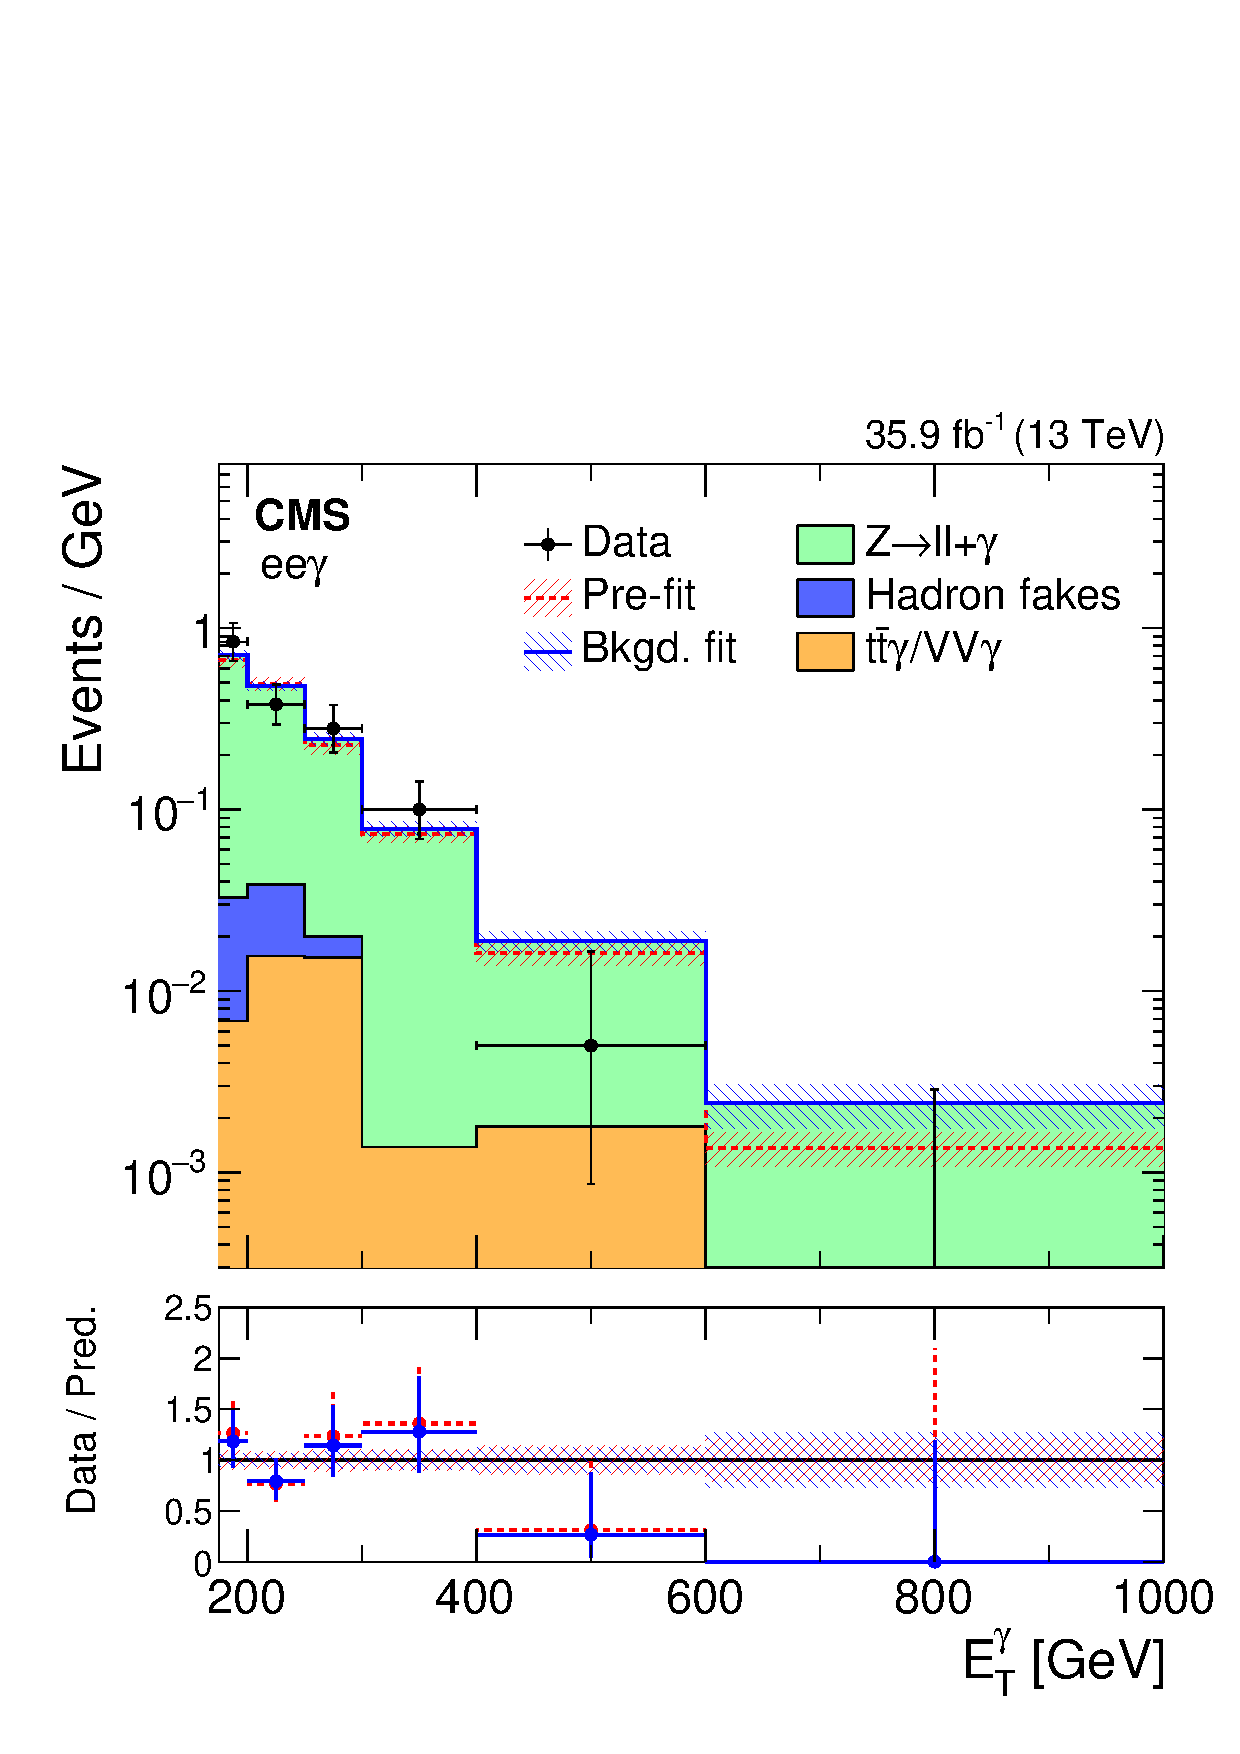
\includegraphics[]{Analysis/Figures/bonly_diel.pdf}
    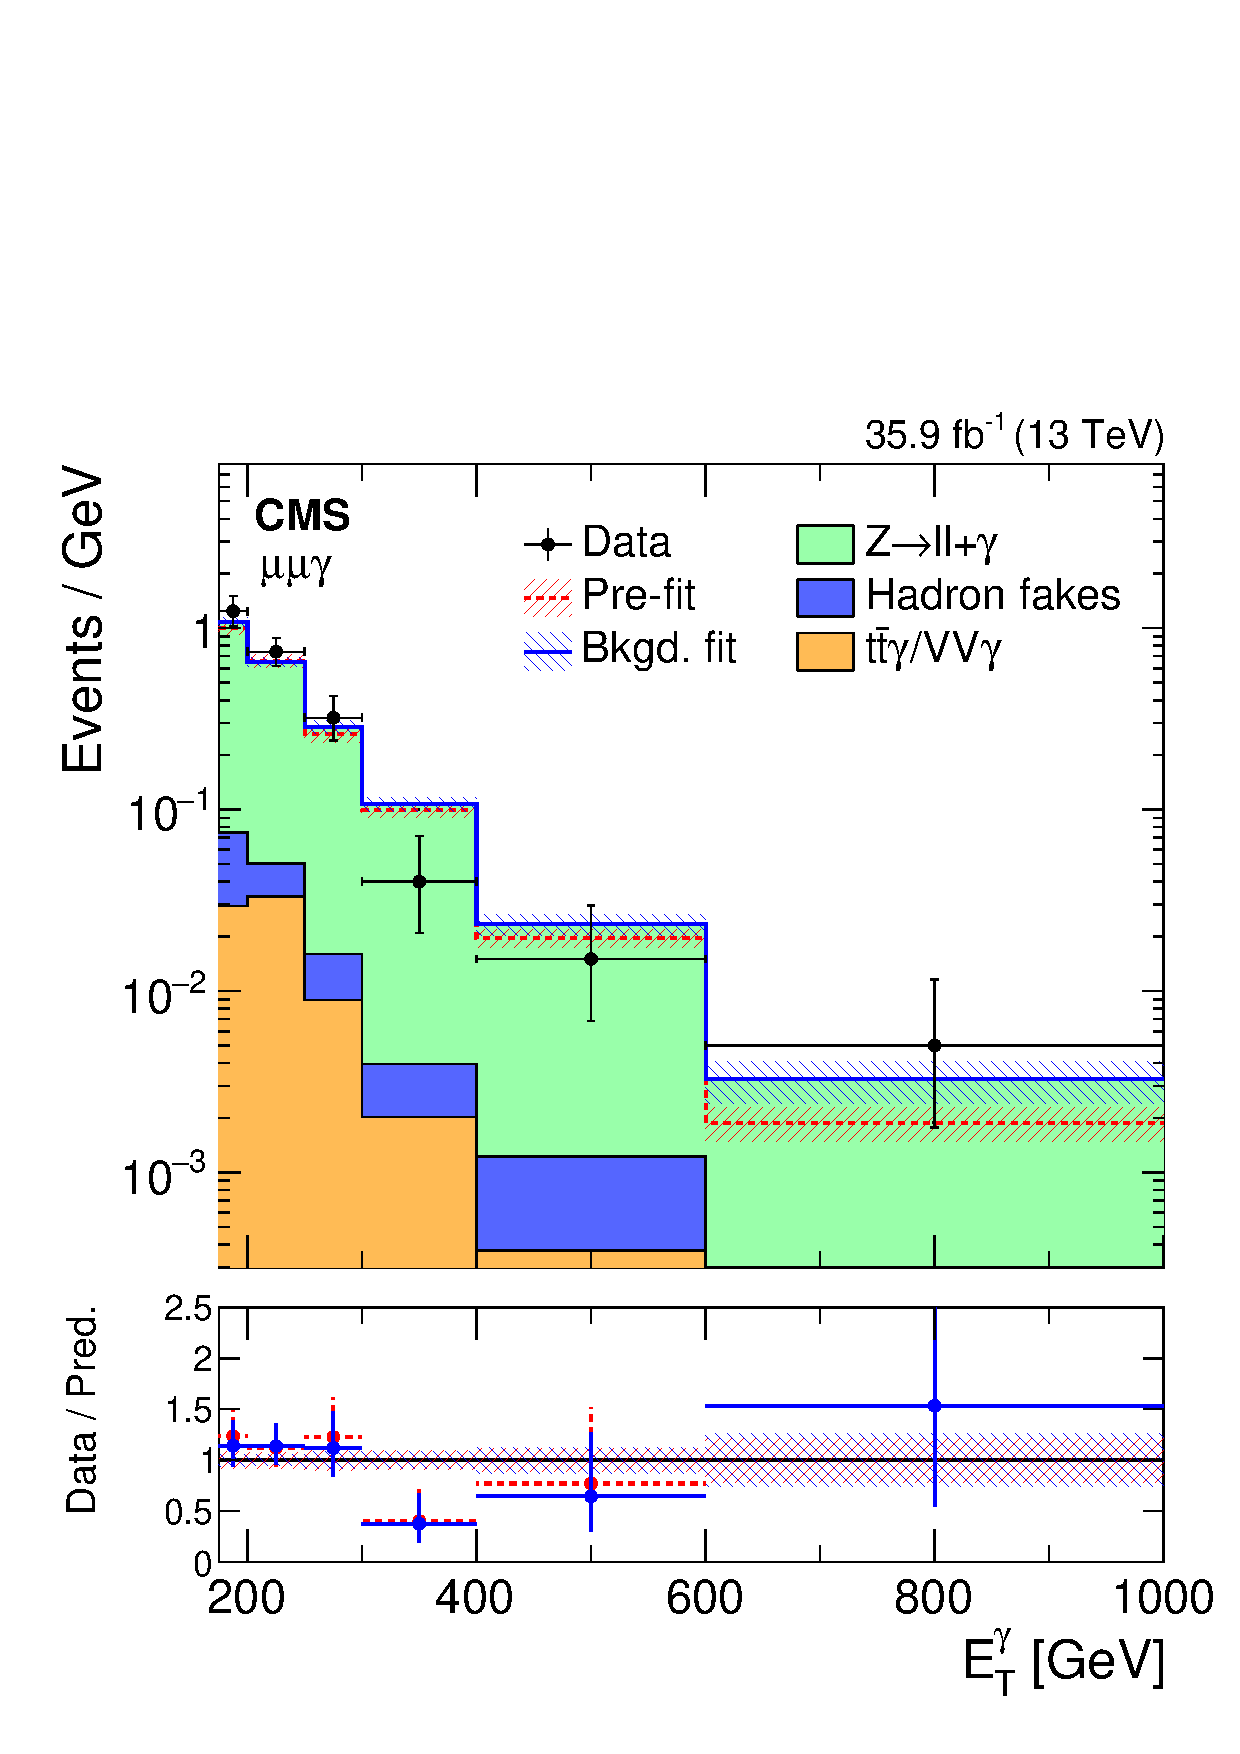
\includegraphics[]{Analysis/Figures/bonly_dimu.pdf}
  }
  \resizebox{\textwidth}{!}{
    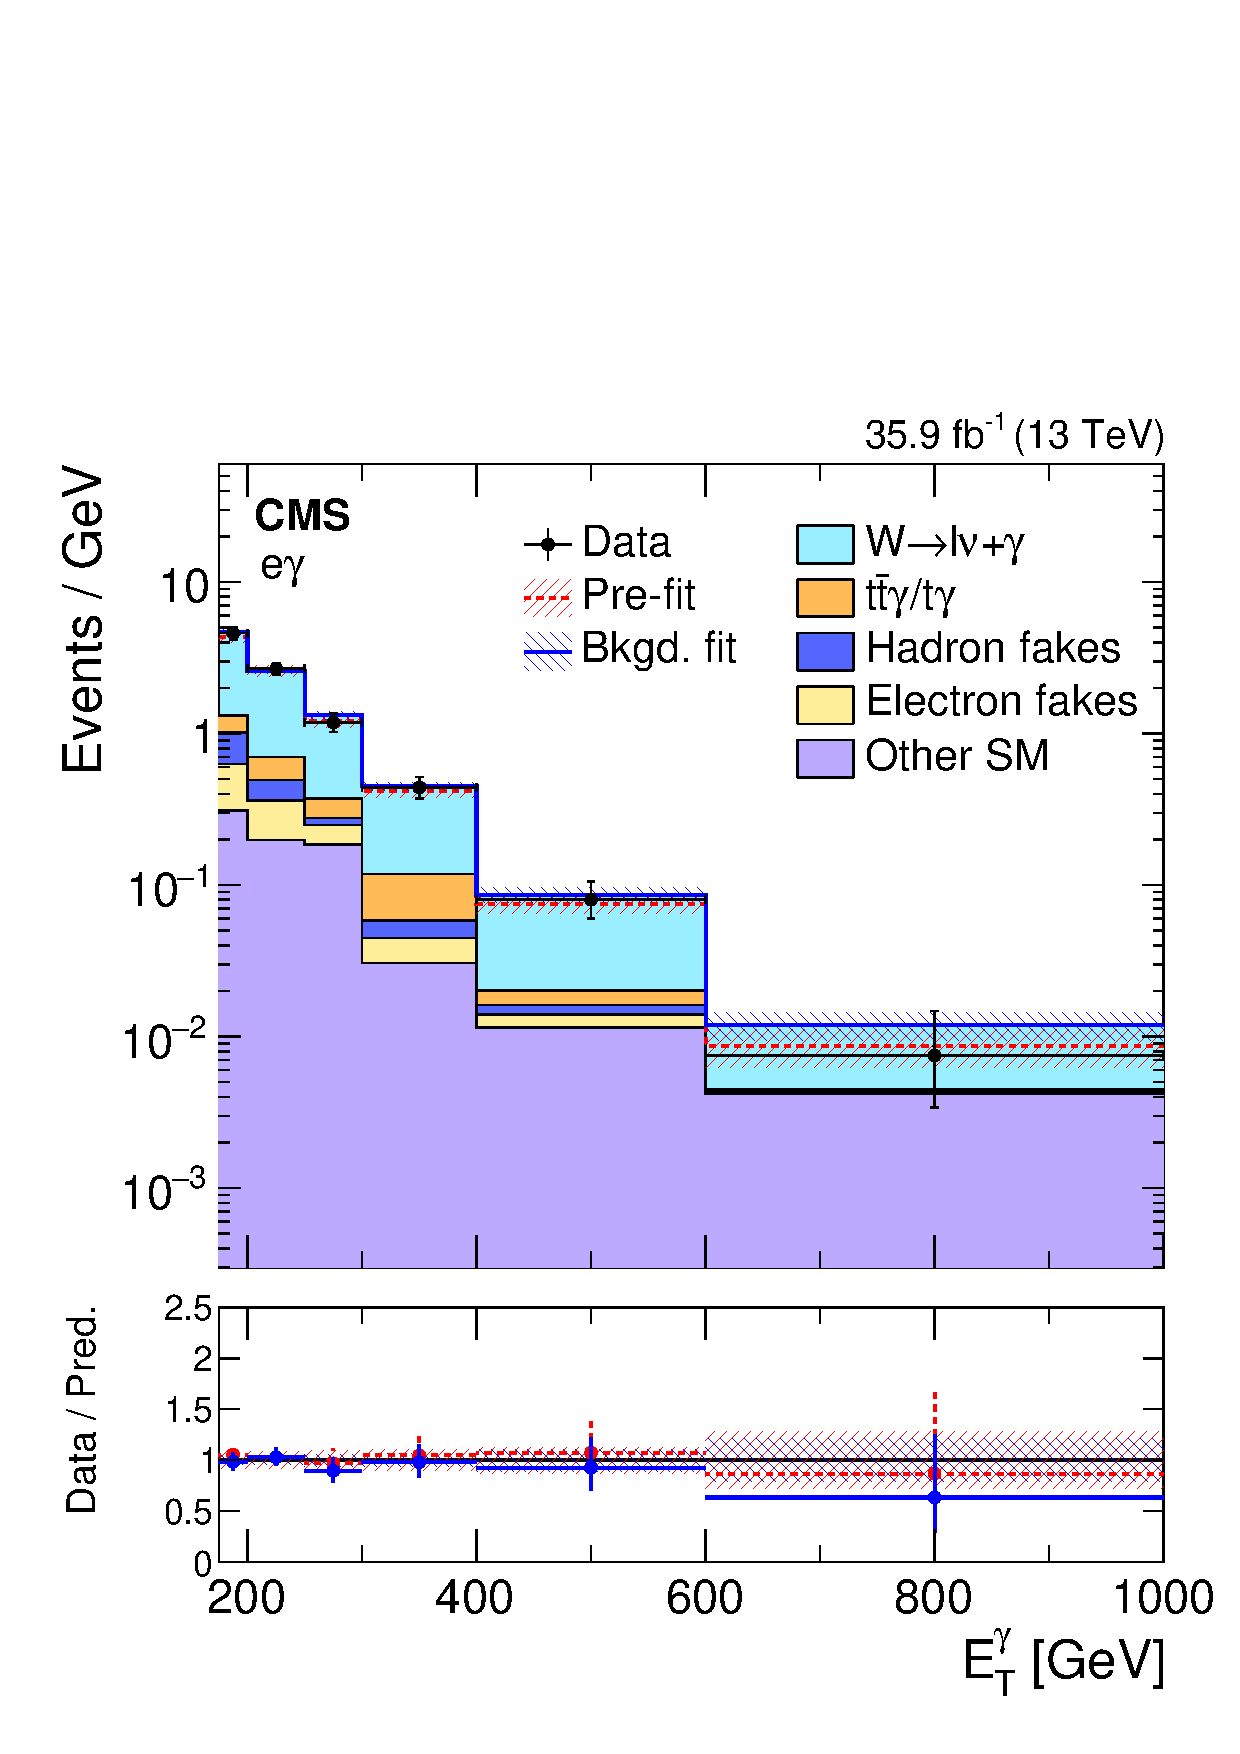
\includegraphics[]{Analysis/Figures/bonly_monoel.pdf}
    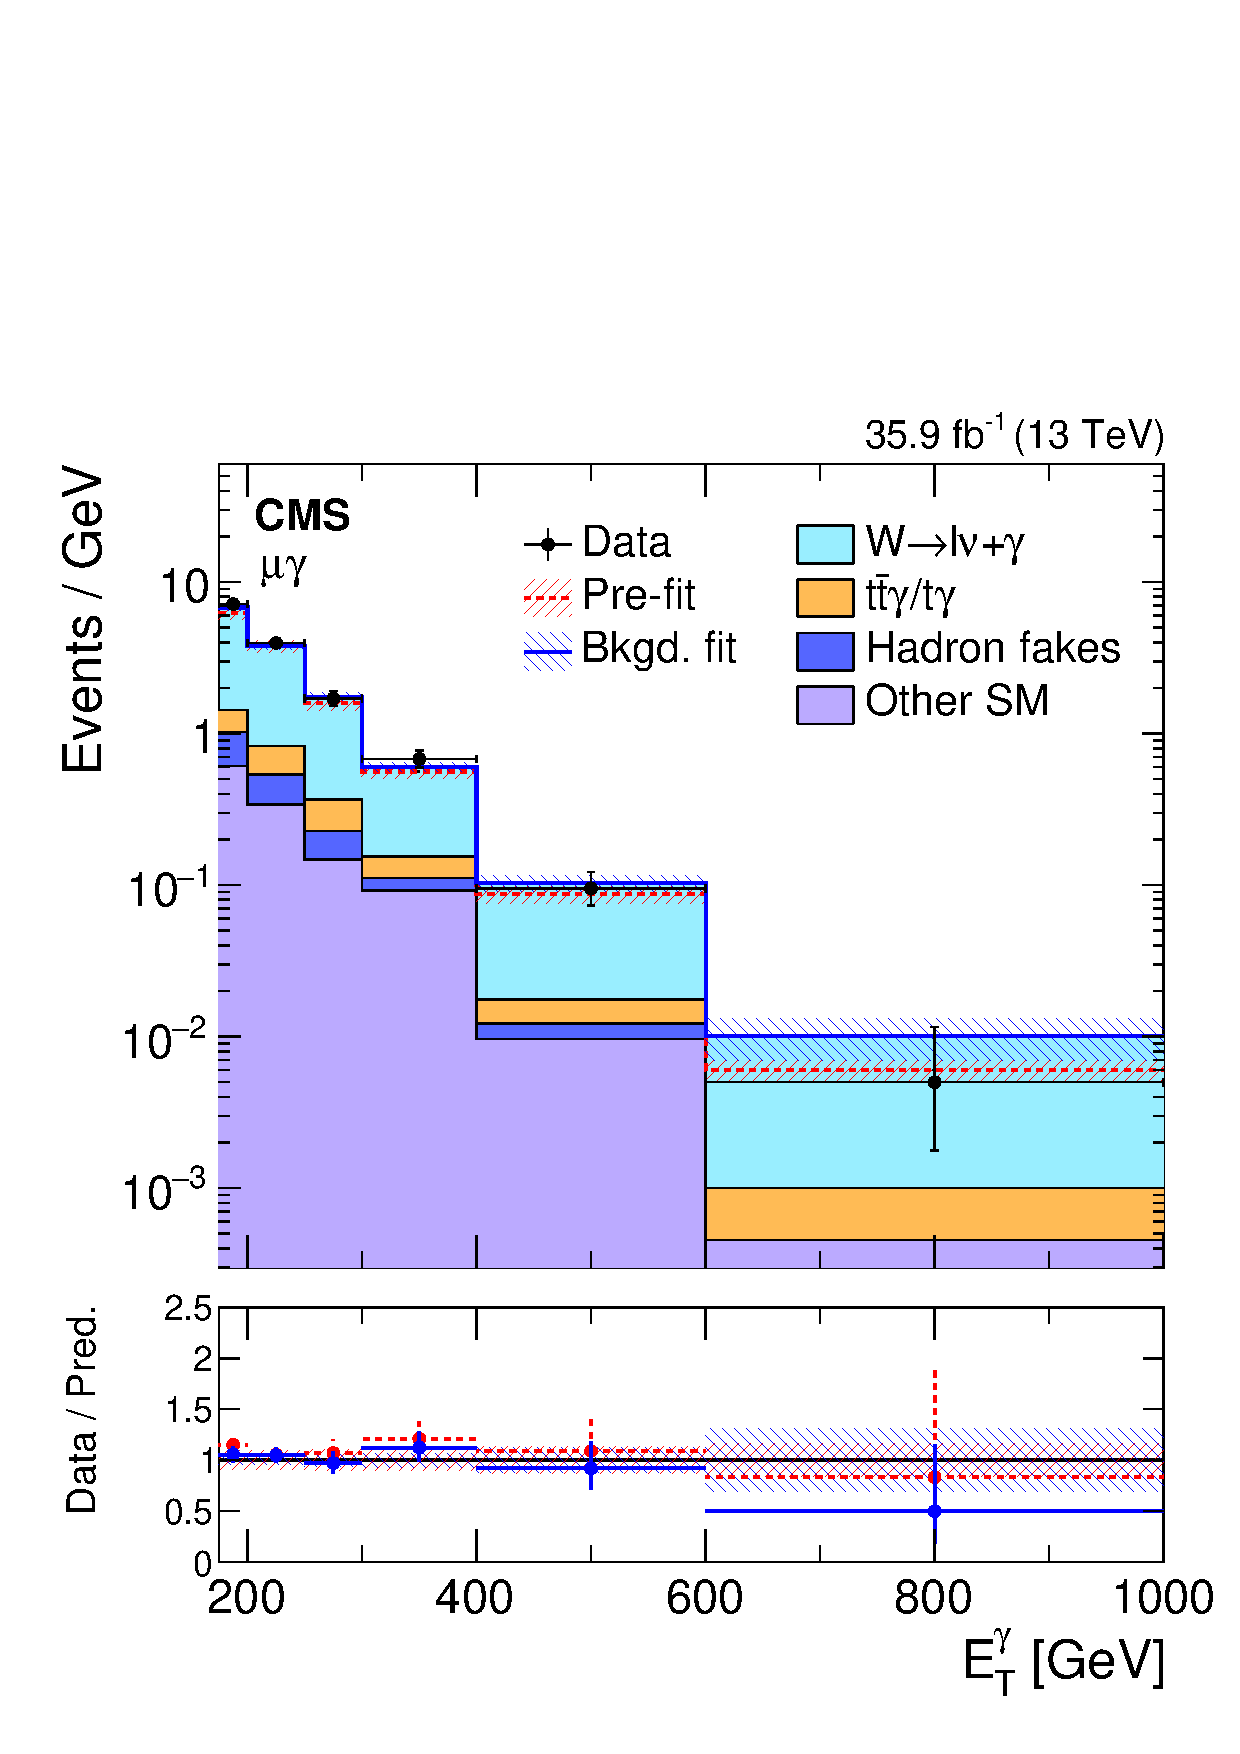
\includegraphics[]{Analysis/Figures/bonly_monomu.pdf}
  }
    \caption{
      Comparison between data and MC simulation in the four control regions: 
      \Pe\Pe\Pgg\ (upper left), 
      \Pgm\Pgm\Pgg\ (upper right), 
      \Pe\Pgg\ (lower left), 
      \Pgm\Pgg\ (lower right) 
      before and after performing the simultaneous fit across all the control samples and signal region, and assuming absence of any signal.
      The last bin of the distribution includes all events with $\ETg > 1000\GeV$. 
      The ratios of data with the pre-fit background prediction (red dashed) and post-fit background prediction (blue solid) are shown in the lower panels. 
      The bands in the lower panels show the post-fit uncertainty after combining all the systematic uncertainties.
}
    \label{fig:postfitCR}
\end{figure}

\subsection{Limits}
\label{sec:limits}

Upper limits are determined for the production cross section of the new-physics processes mentioned in Section~\ref{sec:dm_simp}. 
For each model, a 95\% confidence level (\CL) upper limit is obtained utilizing the asymptotic \CLs\ criterion~\cite{Junk:1999kv,Read:2002hq,Cowan:2010js}, using a test statistic based on the negative logarithm of the likelihood in Section~\ref{sec:interpretation}.

\begin{figure}[htbp]
  \centering
  \resizebox{\textwidth}{!}{
    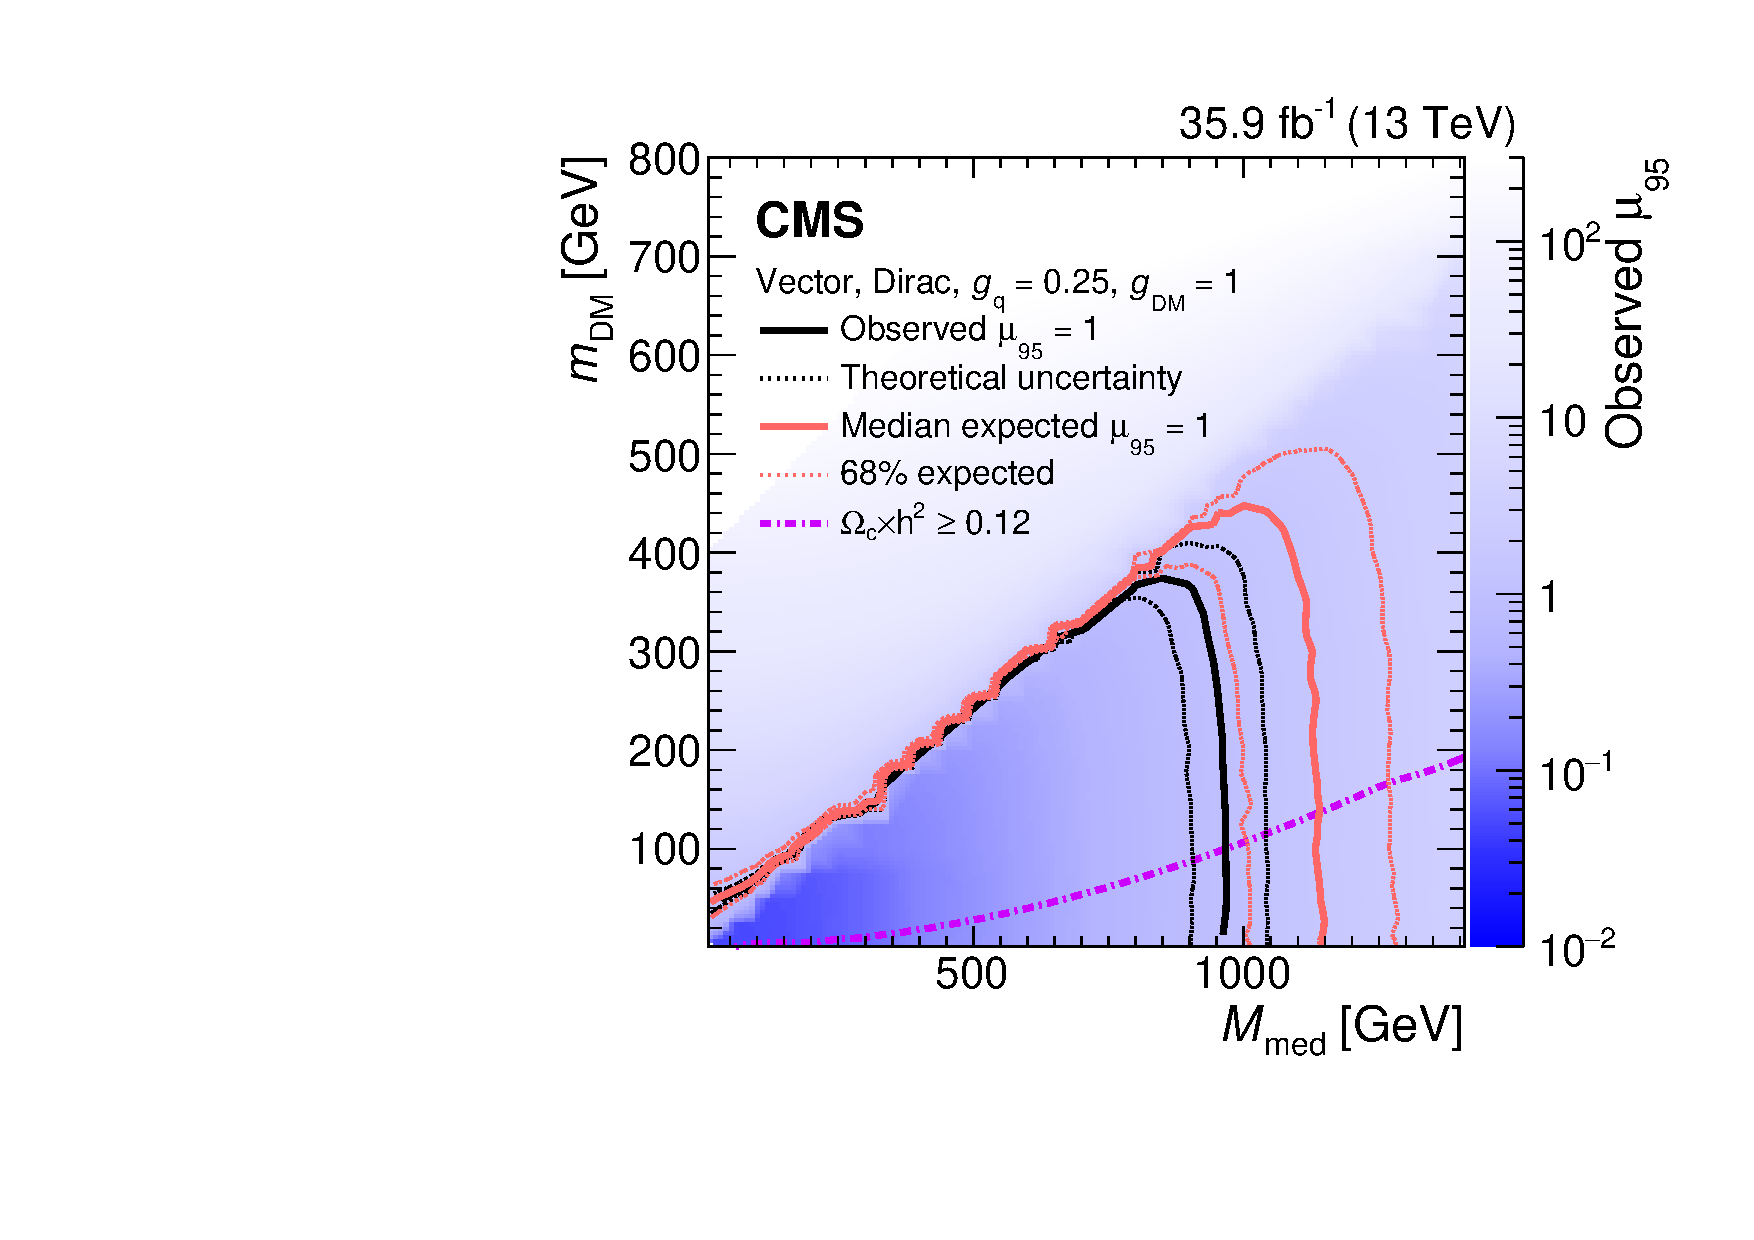
\includegraphics[]{Analysis/Figures/limits_vector.pdf}
    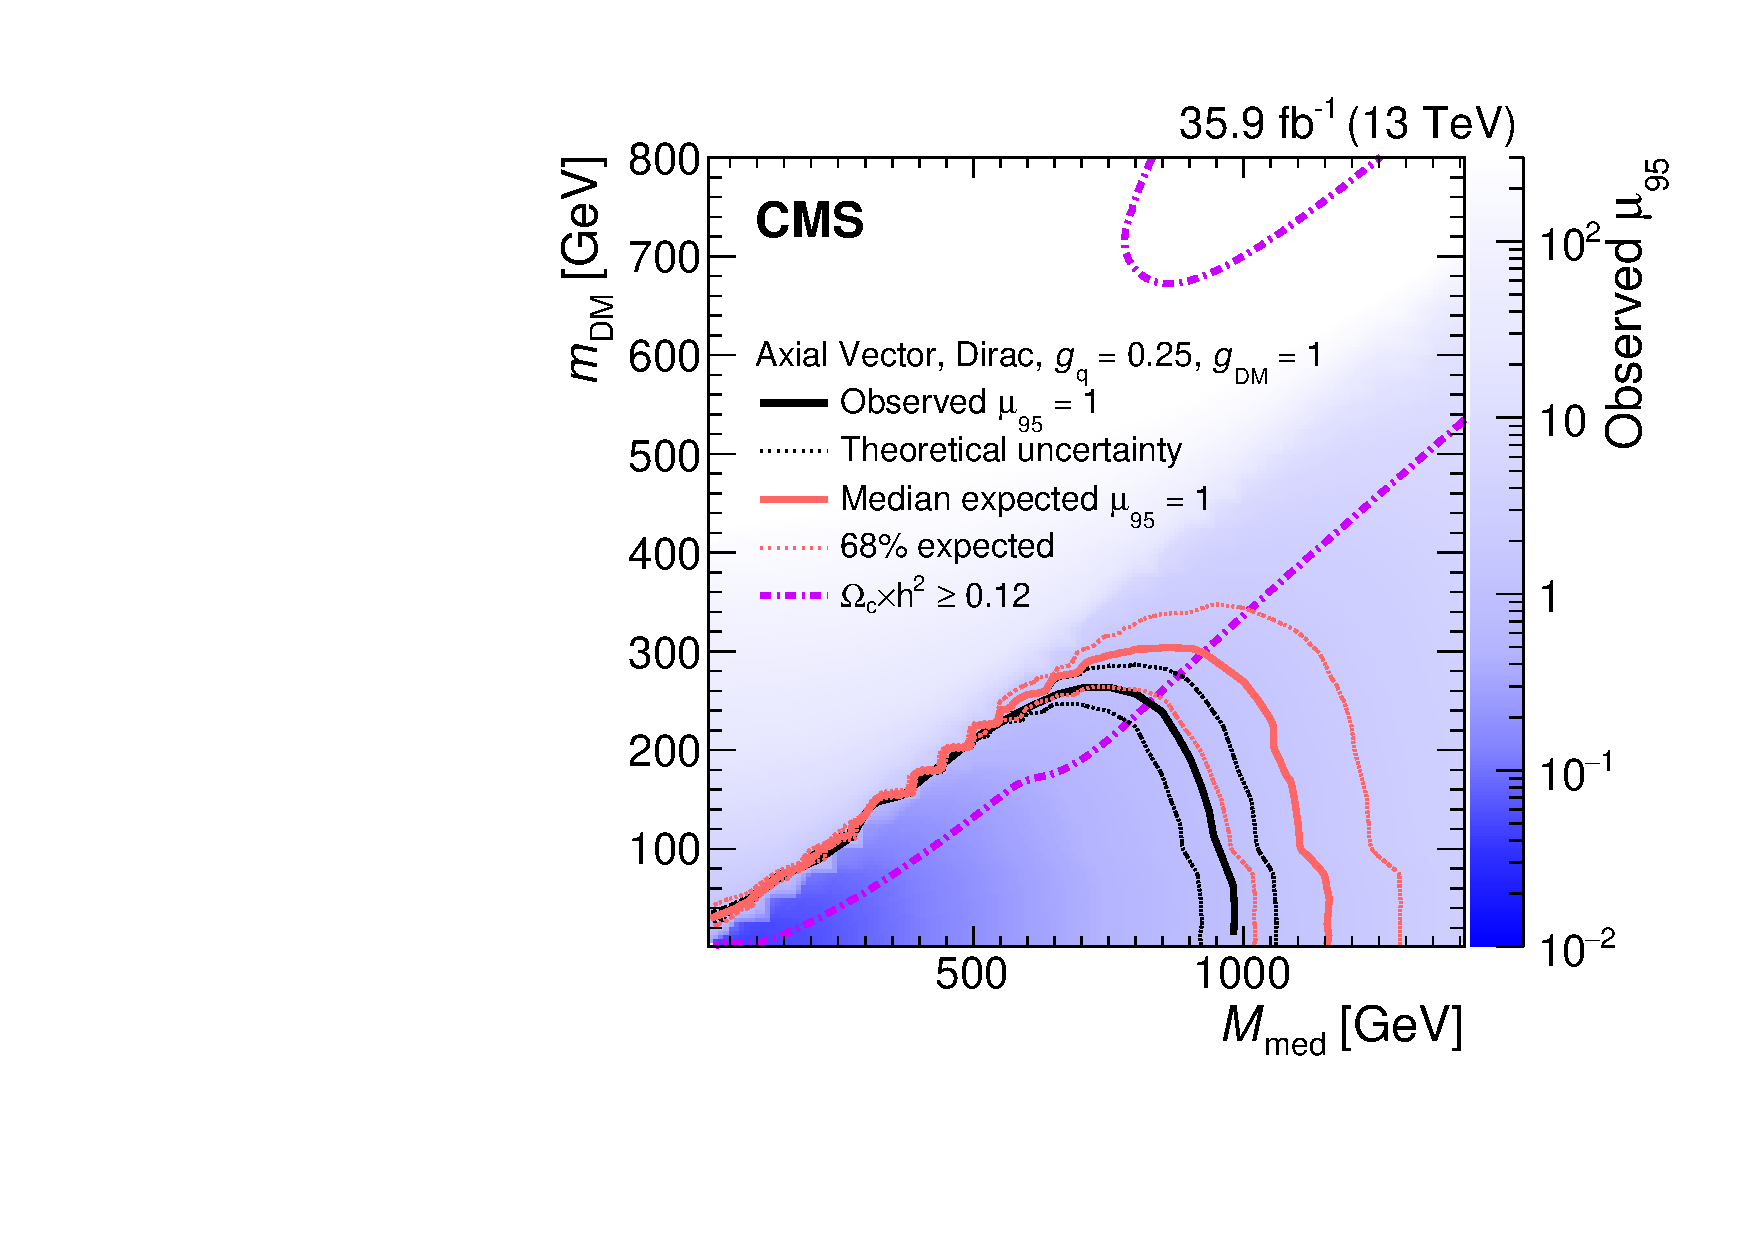
\includegraphics[]{Analysis/Figures/limits_axial.pdf}
  }
  \caption{
    The ratio of 95\% \CL\ upper cross section limits to the theoretical cross section ($\mu_{95}$), for DM simplified models with vector (left) and axial-vector (right) mediators, assuming $\gq=0.25$ and $\gdm=1$.
    The expected $\mu_{95} = 1$ contours are overlaid in red. 
    The region under the observed contour is excluded.
    For DM simplified model parameters in the region below the lower violet dot--dash contour, and also above the corresponding upper contour in the right hand plot, cosmological DM abundance exceeds the density observed by the Planck satellite experiment.
  }
  \label{fig:limits}
\end{figure}

Figure~\ref{fig:limits} shows the 95\% \CL\ upper cross section limits with respect to the corresponding theoretical cross section ($\mu_{95}= \sigma_{95\%}/\sigma_{\text{theory}}$) for the  vector and axial-vector mediator scenarios, in the \mmed--\mdm\ plane. 
The solid black (dashed red) curves are the observed (expected) contours of $\mu_{95} = 1$. 
The $\sigma_{\text{theory}}$ hypothesis is excluded at 95\% \CL\ or above in the region with $\mu_{95} < 1$. 
The uncertainty in the expected upper limit includes the experimental uncertainties. 
For the simplified DM LO models considered, mediator masses up to 950\GeV are excluded for values of \mdm\ less than 1\GeV.

The results for vector and axial-vector mediators are compared to constraints
from the observed cosmological relic density of DM as determined from measurements of the cosmic microwave background by the Planck satellite experiment~\cite{Ade:2015xua}.
The expected DM abundance is estimated, separately for each model, using the thermal freeze-out mechanism implemented in the {\sc MadDM}~\cite{Backovic:2013dpa} framework and  compared to the observed cold DM density $\Omega_c h^2=0.12$~\cite{Ade:2015xua}, where $\Omega_c$ is the DM relic abundance and $h$ is the dimensionless Hubble constant.

\subsection{Comparison to Results from Other Experiments}
\label{sec:comparison}

\begin{figure}[htbp]
  \centering
  \resizebox{\textwidth}{!}{
    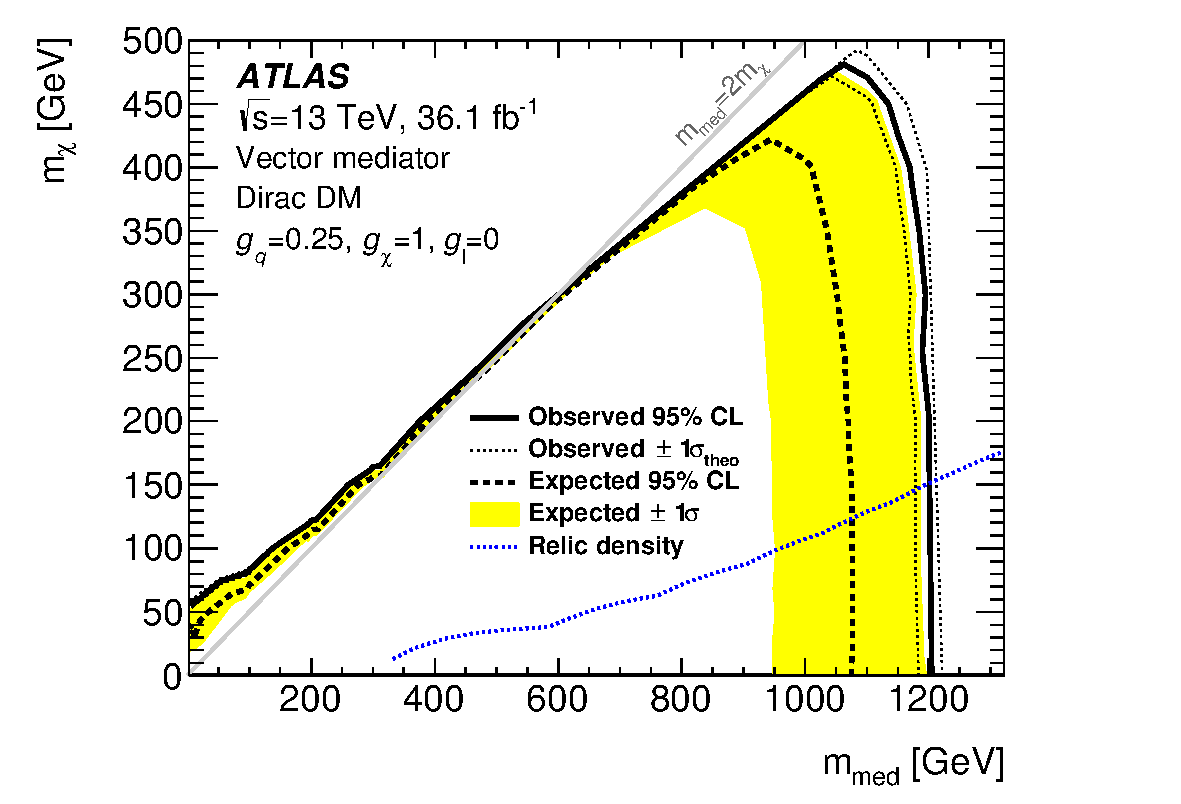
\includegraphics[]{Analysis/Figures/limits_atlas_vector.pdf}
    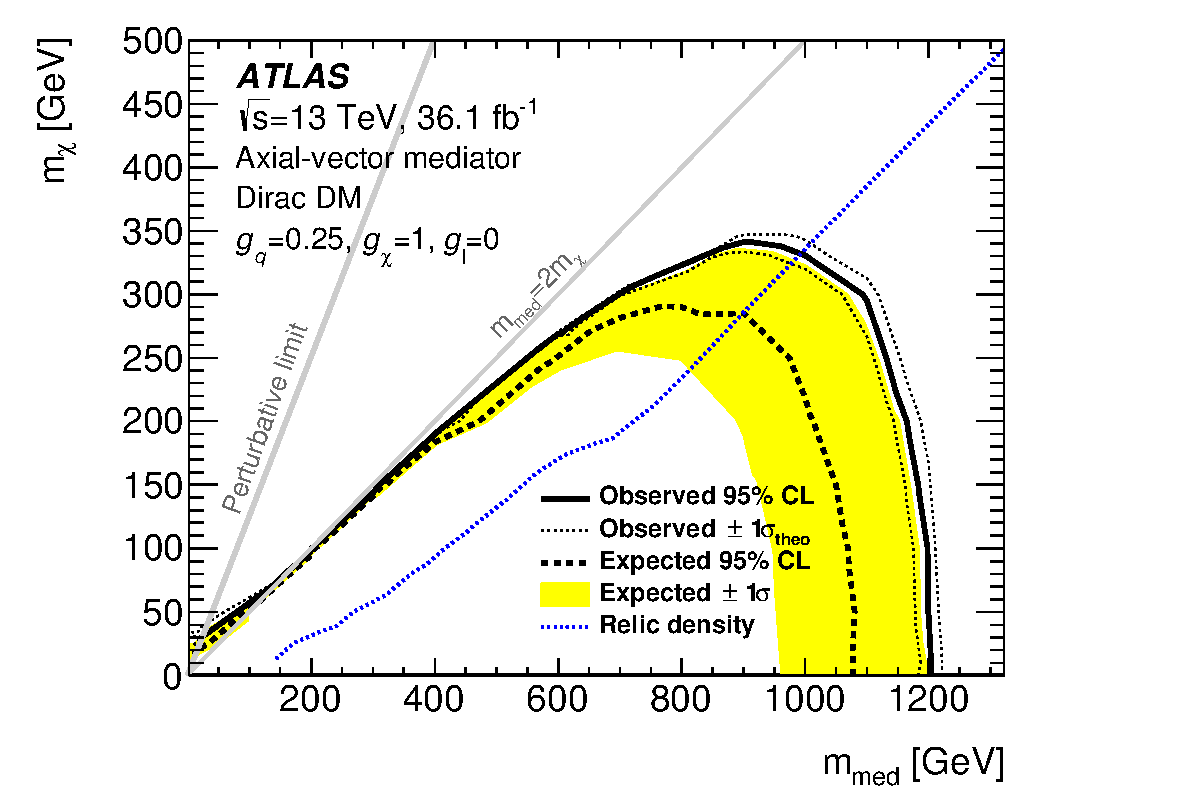
\includegraphics[]{Analysis/Figures/limits_atlas_axial.pdf}
  }
  \caption{
    The equivalent of Figure~\ref{fig:limits} with results from ATLAS.
    The expected $\mu_{95} = 1$ contours are overlaid in yellow. 
    The region under the observed contour is excluded.
    Reprinted from Reference~\cite{ATLAS2017} 
    % https://atlas.web.cern.ch/Atlas/GROUPS/PHYSICS/PAPERS/EXOT-2016-32/
  }
  \label{fig:limits_atlas}
\end{figure}

The results from an equivalent analysis by ATLAS~\cite{ATLAS2017} are shown in Figure~\ref{fig:limits_atlas}.
%% need to descibe

\begin{figure}[htbp]
  \centering
  \resizebox{\textwidth}{!}{
    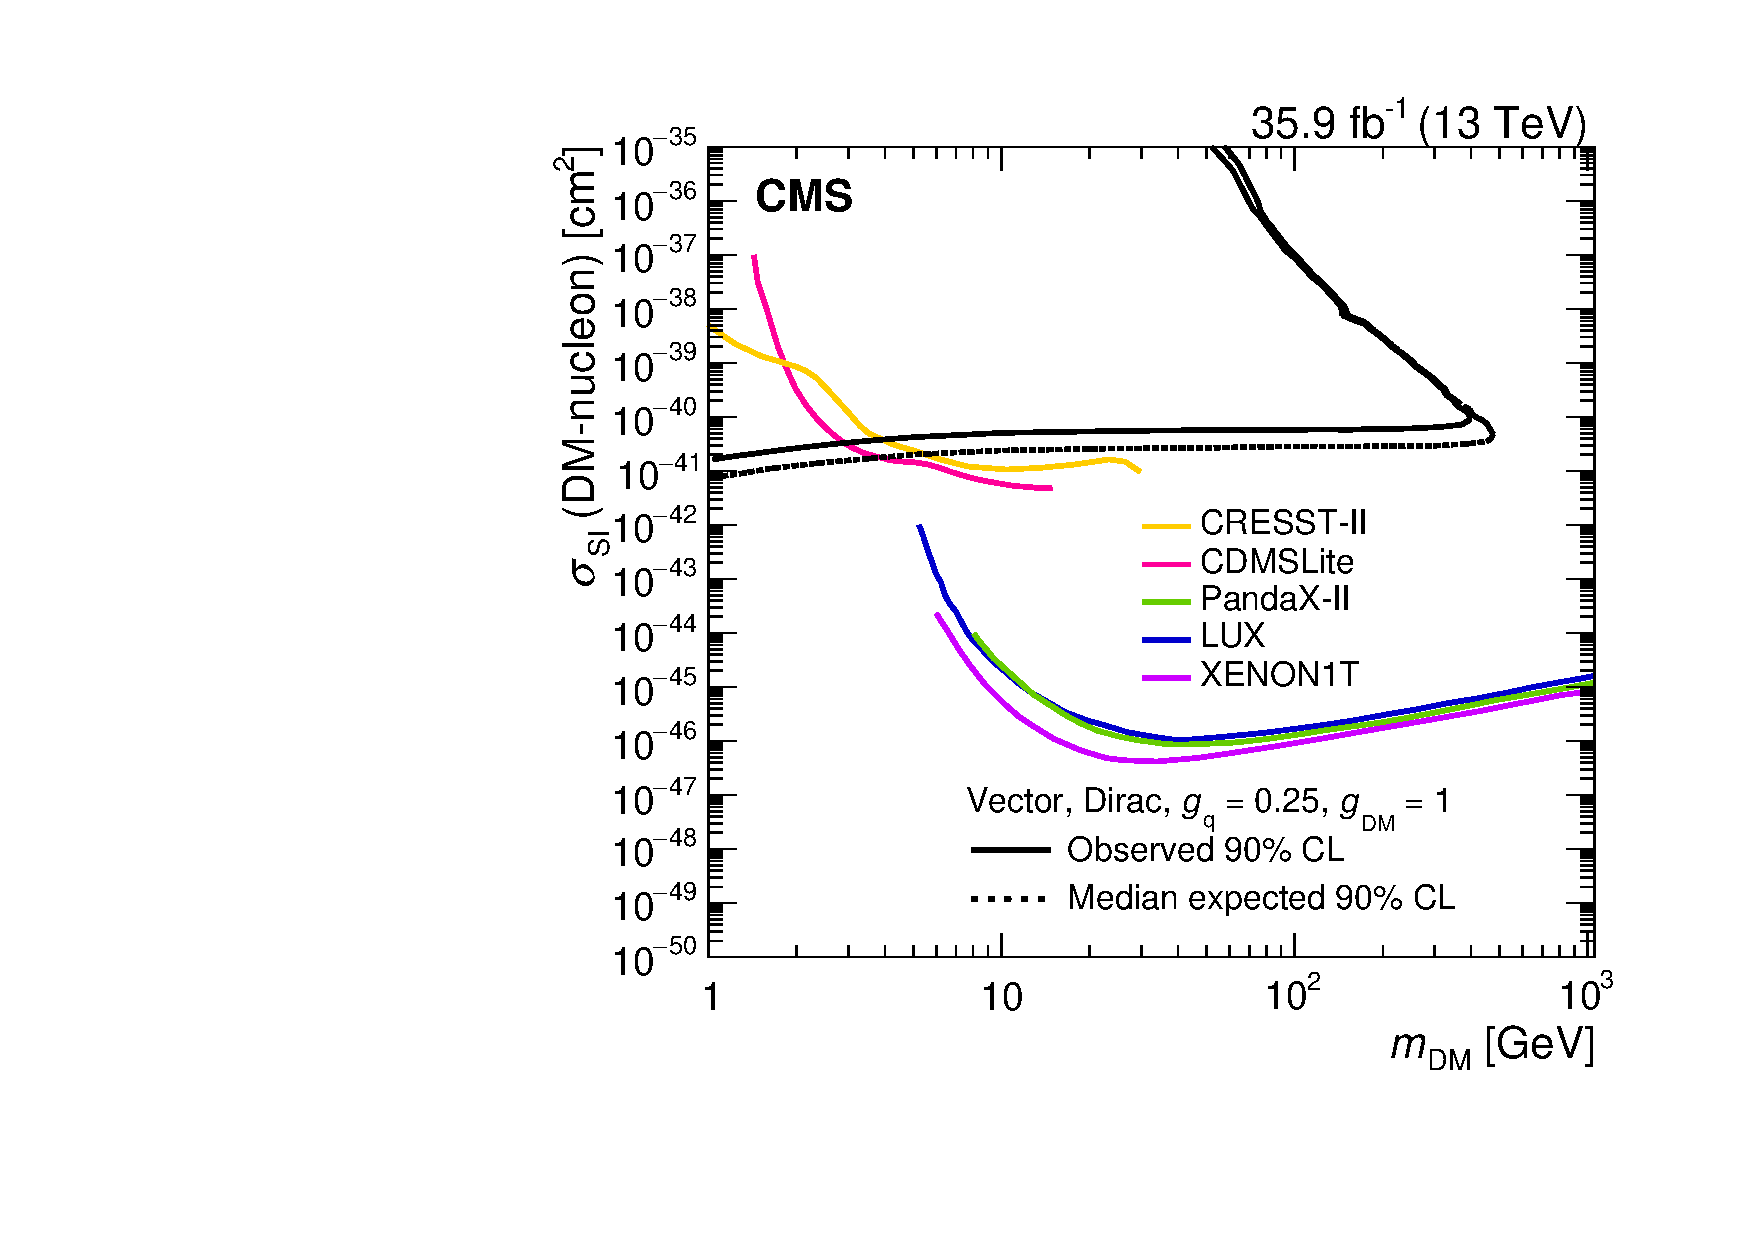
\includegraphics[]{Impact/Figures/limits_direct.pdf}
    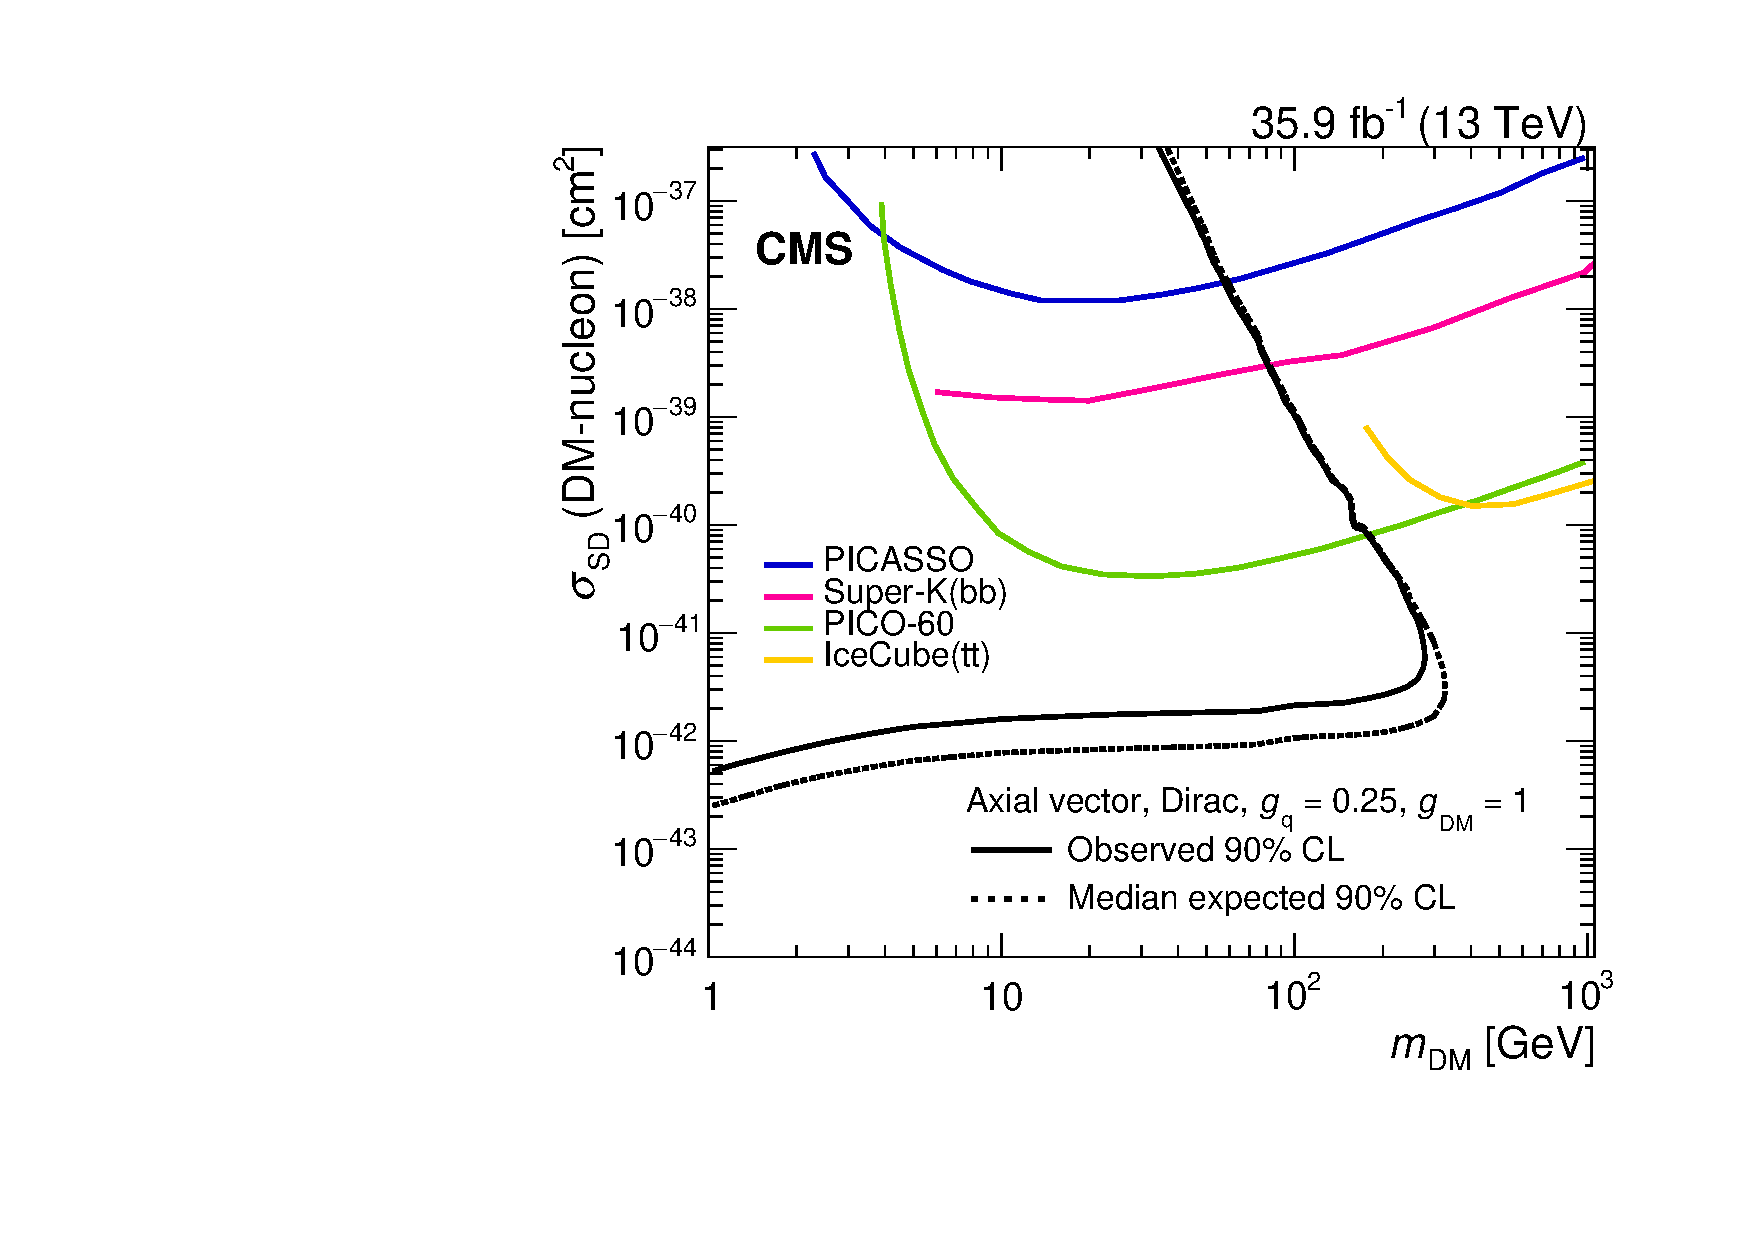
\includegraphics[]{Impact/Figures/limits_indirect.pdf}
  }
  \caption{
    The 90\% \CL\ exclusion limits on the $\chi$--nucleon spin-independent scattering cross sections involving the vector operator (top) and the $\chi$--nucleon spin-dependent scattering cross sections involving the axial-vector operator (bottom) as a function of the \mdm.
    Simplified model DM parameters of $\gq=0.25$ and $\gdm=1$ are assumed.
    The region to the upper left of the contour is excluded. 
    On the plots, the median expected 90\% \CL\ curve overlaps the observed 90\% \CL\ curve.
    Also shown are corresponding exclusion contours, where regions above the curves are excluded, from the recent results by the direct and indirect detection experiments listed in the text.
    }
    \label{fig:limits_direct}
\end{figure}

To enable a direct comparison with results from direct and indirect detection experiments, the 95\% \CL limits on the mediator mass for the vector and axial-vector models are translated to 90\% \CL limits on the spin-independent and spin-dependent DM--nucleon scattering cross sections, $\sigma_{\text{SI}}$ and $\sigma_{\text{SD}}$ respectively, following the prescriptions given in Reference~\cite{Boveia:2016mrp} and~\cite{DMF2015}.
The exclusion contours for the vector and axial-vector models shown in Figure~\ref{fig:limits} are translated into the $\sigma_{\text{SI}}$--\mdm\ and $\sigma_{\text{SD}}$--\mdm\ planes shown in Figure~\ref{fig:limits_direct}. 
When compared to recent results by the CDMSLite~\cite{CDMS2016}, LUX~\cite{LUX2017}, PandaX-II~\cite{Cui:2017}, XENON1T~\cite{Aprile:2018}, and CRESST-II~\cite{Angloher:2015ewa} collaborations, the limits obtained from this search provide stronger constraints for DM masses less than 2\GeV for spin independent models.
When compared to recent results by the PICO-60~\cite{PICO2017}, IceCube~\cite{IceCube2016}, PICASSO~\cite{Behnke:2016lsk} and Super-Kamiokande~\cite{Choi:2015ara} collaborations, the limits obtained from this search provide stronger constraints for DM masses less than 200\GeV for spin dependent models.

\subsection{Interpretation of Additional Models}
\label{sec:reinterpretation}

In addition to the background-only fit to all of the signal and control regions, we performed a simultaneous maximum likelihood fit to the observed \ETg\ distributions in the control regions only.
The results of this fit enable the interpretation of new physics models not studied in this thesis with the simplified likelihood approach detailed in Reference~\cite{CMS-NOTE-2017-001}.
The predicted yields in each bin of \ETg\ for all backgrounds in the horizontal and vertical signal regions after performing the control region only fit are given in Tables~\ref{tab:yield_mask_horizontal} and~\ref{tab:yield_mask_vertical}, respectively.
The covariances between the predicted background yields across all the \ETg~bins in the two signal regions are shown in Fig.~\ref{fig:correlation_matrix}.

\begin{table}[htbp]
  \centering
  \resizebox{\textwidth}{!}{
\begin{tabular}{ l|cccccc }
\rule[-1.2ex]{0pt}{3.8ex}\ETg~[\GeVns{}]      &         [175,  200] &         [200,  250] &         [250,  300] &         [300,  400] &         [400,  600] &         [600, 1000] \\
\hline
$\PZ\Pgg$        & $  81.2 \pm   8.0 $ & $  88.2 \pm   8.4 $ & $  38.8 \pm   4.8 $ & $  26.8 \pm   3.7 $ & $   8.8 \pm   1.9 $ & $   1.4 \pm   0.7 $ \\
$\PW\Pgg$        & $  27.9 \pm   3.7 $ & $  29.9 \pm   3.9 $ & $  11.4 \pm   1.7 $ & $   6.3 \pm   1.2 $ & $   1.4 \pm   0.4 $ & $   0.1 \pm   0.1 $ \\
Misid. electrons & $  22.5 \pm   2.7 $ & $  25.7 \pm   2.7 $ & $  10.5 \pm   1.0 $ & $   8.2 \pm   0.7 $ & $   2.7 \pm   0.2 $ & $   0.5 \pm   0.0 $ \\
Misid. hadrons   & $   5.2 \pm   2.2 $ & $   9.3 \pm   1.8 $ & $   3.1 \pm   0.7 $ & $   1.0 \pm   0.3 $ & $   0.4 \pm   0.1 $ & $   0.0 \pm   0.0 $ \\
Other SM         & $  13.6 \pm   2.0 $ & $  19.6 \pm   1.3 $ & $  13.9 \pm   0.4 $ & $   4.2 \pm   0.2 $ & $   0.8 \pm   0.0 $ & $   0.1 \pm   0.0 $ \\
ECAL spikes      & $   4.3 \pm   1.3 $ & $   2.7 \pm   0.8 $ & $   0.5 \pm   0.1 $ & $   0.1 \pm   0.0 $ & $   0.0 \pm   0.0 $ & $   0.0 \pm   0.0 $ \\
Total prediction & $ 154.6 \pm   8.3 $ & $ 175.4 \pm   8.8 $ & $  78.2 \pm   5.3 $ & $  46.6 \pm   4.0 $ & $  14.1 \pm   2.1 $ & $   2.1 \pm   0.8 $ \\
\hline
Observed         & $ 150   \pm  12   $ & $ 166   \pm    13 $ & $  76.0 \pm   8.7 $ & $  44.0 \pm   6.6 $ & $  19.0 \pm   4.4 $ & $   4.0 \pm   2.0 $ \\
\end{tabular}
}
\caption{Expected event yields in each \ETg\ bin for the various background processes in \underline{\textbf{the horizontal signal region}}.
         The background yields and the corresponding uncertainties are obtained after performing a combined fit to data in all the control samples, excluding data in the signal region.
         The observed event yields in the horizontal signal region are also reported.}
\label{tab:yield_mask_horizontal}
\end{table}

\begin{table}[htbp]
  \centering
  \resizebox{\textwidth}{!}{
\begin{tabular}{ l|cccccc }
\rule[-1.2ex]{0pt}{3.8ex}\ETg~[\GeVns{}]      &         [175,  200] &         [200,  250] &         [250,  300] &         [300,  400] &         [400,  600] &         [600, 1000] \\
\hline
$\PZ\Pgg$        & $ 172   \pm    17 $ & $ 190   \pm  18   $ & $  83   \pm  10   $ & $  58.6 \pm   7.9 $ & $  18.0 \pm   3.9 $ & $   3.1 \pm   1.6 $ \\
$\PW\Pgg$        & $  59.9 \pm   7.8 $ & $  63.6 \pm   7.8 $ & $  24.6 \pm   3.5 $ & $  13.4 \pm   2.4 $ & $   3.0 \pm   0.8 $ & $   0.3 \pm   0.2 $ \\
Misid. electrons & $  48.4 \pm   5.6 $ & $  56.2 \pm   5.1 $ & $  23.4 \pm   1.8 $ & $  15.7 \pm   1.4 $ & $   5.6 \pm   0.4 $ & $   1.2 \pm   0.1 $ \\
Misid. hadrons   & $  15.1 \pm   4.4 $ & $  14.5 \pm   3.1 $ & $   4.2 \pm   0.8 $ & $   2.3 \pm   0.8 $ & $   0.5 \pm   0.1 $ & $   0.1 \pm   0.1 $ \\
Other SM         & $  33.8 \pm   4.1 $ & $  36.6 \pm   2.7 $ & $  13.6 \pm   0.5 $ & $  17.1 \pm   0.6 $ & $   2.4 \pm   0.1 $ & $   0.8 \pm   0.0 $ \\
ECAL spikes      & $   9.3 \pm   2.8 $ & $   5.7 \pm   1.7 $ & $   0.9 \pm   0.3 $ & $   0.3 \pm   0.1 $ & $   0.0 \pm   0.0 $ & $   0.0 \pm   0.0 $ \\
Total prediction & $ 339   \pm  18  $ & $ 366   \pm  19   $ & $ 150   \pm  11   $ & $ 107.5 \pm   8.7 $ & $  29.6 \pm   4.3 $ & $   5.4 \pm   1.7 $ \\
\hline
Observed         & $ 301   \pm  17   $ & $ 342   \pm  19   $ & $ 161 \pm  13   $ & $ 107   \pm  10   $ & $  41.0 \pm   6.4 $ & $  12.0 \pm   3.5 $ \\
\end{tabular}
}
\caption{Expected event yields in each \ETg\ bin for the various background processes in  \underline{\textbf{the vertical signal region}}.
         The background yields and the corresponding uncertainties are obtained after performing a combined fit to data in all the control samples, excluding data in the signal regions.
         The observed event yields in the vertical signal region are also reported.}
\label{tab:yield_mask_vertical}
\end{table}

\begin{figure}[hbtp]
  \centering
  \resizebox{\textwidth}{!}{
    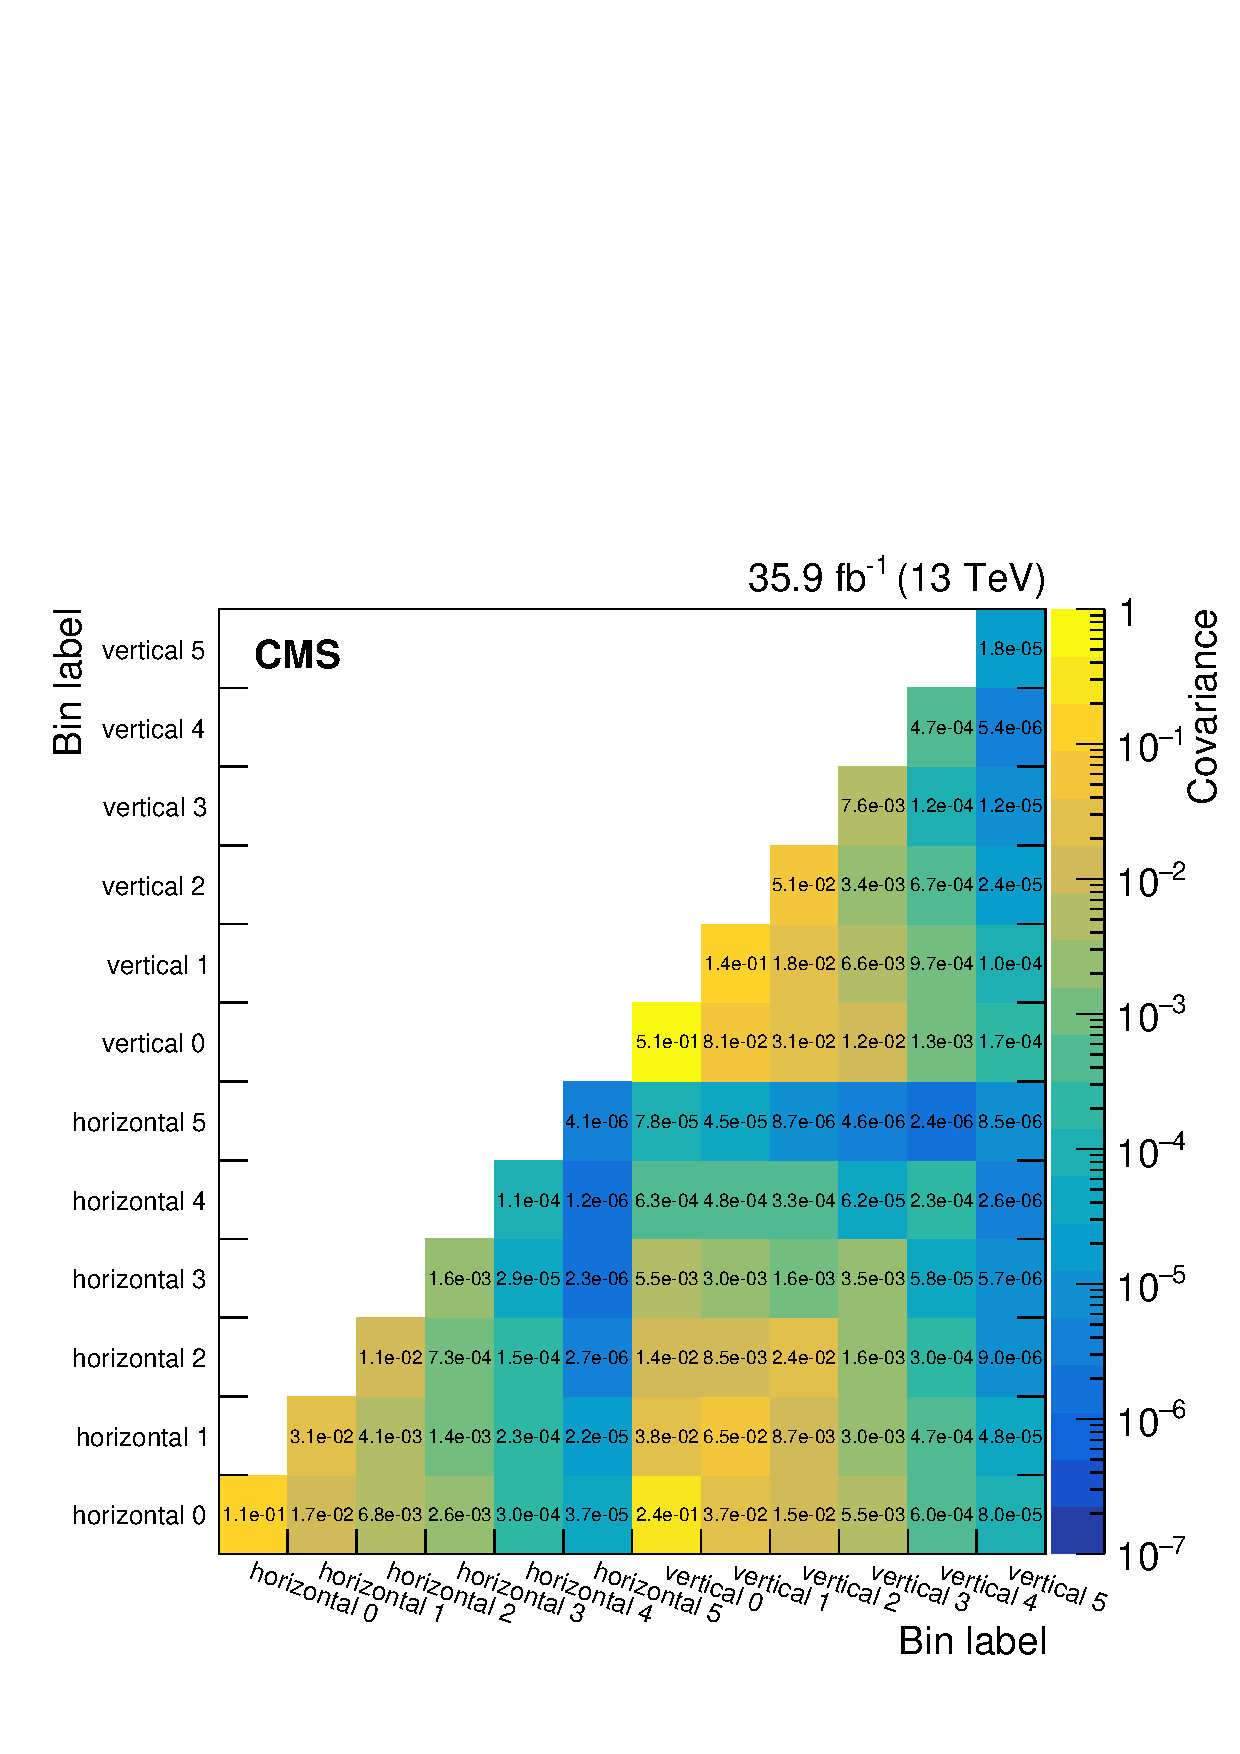
\includegraphics[]{Analysis/Figures/correlation_matrix.pdf}
  }
  \caption{
    Covariances between the predicted background yields in all the \ETg\ bins of the horizontal and vertical signal regions.
    The bin labels specify which signal region the bin belongs to and what number bin it is for that region.}
  \label{fig:correlation_matrix}
\end{figure}.
